\documentclass[tikz]{standalone}

\usetikzlibrary{arrows.meta}
\tikzset{>=stealth}

\begin{document}
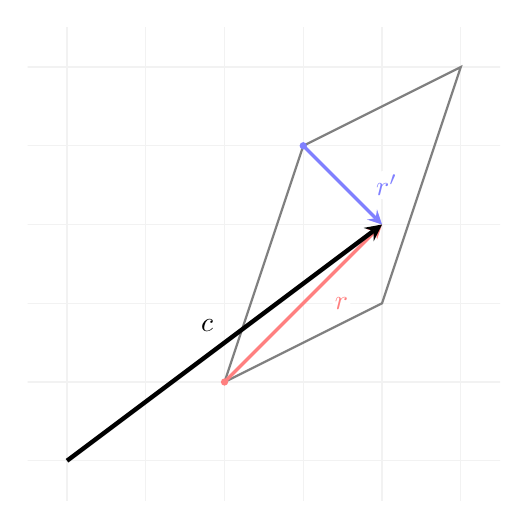
\begin{tikzpicture}
  \clip (-0.5, -0.5) rectangle (5.5, 5.5);
  \draw[black!5] (-4, -3) grid (11, 8);
  %\draw (0, 0) -- ++(2, 1) -- ++(1, 3) -- ++(-2, -1) -- ++(-1, -3);
  \draw[black!50, thick] (2,1) -- ++(2, 1) -- ++(1, 3) -- ++(-2, -1) -- ++(-1, -3);
  \draw[->,very thick, red!50]  (2, 1) -- node[right=1em, fill=white, inner sep=0pt, circle] {$r$} (4, 3);
  \draw[->,very thick, blue!50] (3, 4) -- node[right=1em, fill=white, inner sep=0pt, circle] {$r'$} (4, 3);
  \draw[->, ultra thick] (0, 0) -- node[above left] {$c$} (4,3);

  \draw[red!50, fill] (2, 1) circle (1.1pt);
  \draw[blue!50, fill] (3, 4) circle (1.1pt);
\end{tikzpicture}
\end{document}
